\documentclass[border=4pt]{standalone}
\usepackage{amsmath,amssymb,tikz}
\usetikzlibrary{arrows.meta,calc,matrix,positioning}
\definecolor{figB}{RGB}{31,90,166}\definecolor{figR}{RGB}{176,48,48}\definecolor{figG}{RGB}{46,125,50}\definecolor{figO}{RGB}{214,120,20}
\begin{document}
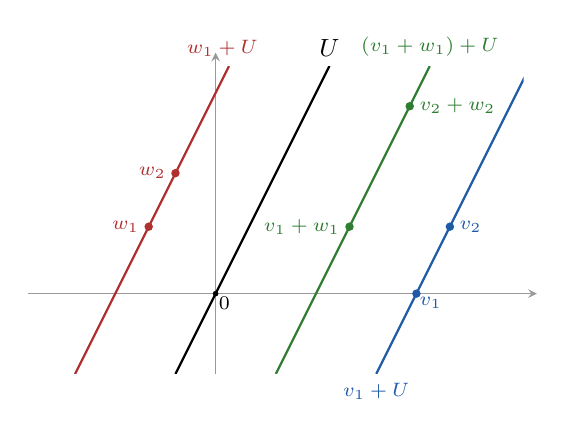
\begin{tikzpicture}[scale=0.85,>={Stealth[length=2mm]}]
\draw[-stealth,thin,black!40] (-2.8,0)--(4.8,0);
\draw[-stealth,thin,black!40] (0,-1.2)--(0,3.6);
\begin{scope}
\clip (-2.8,-1.2) rectangle (4.6,3.4);
\draw[black,thick] (-0.6,-1.2)--(1.7,3.4);            % U: y=2x
\draw[figR,thick] (-2.1,-1.2)--(0.2,3.4);             % w1+U: y=2x+3
\draw[figG,thick] (0.9,-1.2)--(3.2,3.4);              % (v1+w1)+U: y=2x-3
\draw[figB,thick] (2.4,-1.2)--(4.7,3.4);              % v1+U: y=2x-6
\end{scope}
\node[font=\small,anchor=south] at (1.7,3.4) {$U$};
\node[font=\scriptsize,figR,anchor=south] at (0.1,3.4) {$w_1+U$};
\node[font=\scriptsize,figG,anchor=south] at (3.2,3.4) {$(v_1+w_1)+U$};
\node[font=\scriptsize,figB,anchor=north] at (2.4,-1.2) {$v_1+U$};
\fill[figB] (3,0) circle (1.8pt) node[below right,font=\scriptsize,inner sep=1pt]{$v_1$};
\fill[figB] (3.5,1) circle (1.8pt) node[right,font=\scriptsize]{$v_2$};
\fill[figR] (-1,1) circle (1.8pt) node[left,font=\scriptsize]{$w_1$};
\fill[figR] (-0.6,1.8) circle (1.8pt) node[left,font=\scriptsize]{$w_2$};
\fill[figG] (2,1) circle (1.8pt) node[left,font=\scriptsize]{$v_1+w_1$};
\fill[figG] (2.9,2.8) circle (1.8pt) node[right,font=\scriptsize]{$v_2+w_2$};
\fill (0,0) circle (1.2pt) node[below right,font=\scriptsize,inner sep=1pt]{$0$};
\end{tikzpicture}
\end{document}
